\chapter{Codifica} \label{chap:codifica}
	
	Iniziamo finalmente l'analisi dell'algoritmo di compressione MP3. I passi principali di quest'algoritmo sono illustrati in Figura \ref{fig:encode_layout}.\\
	
	\begin{figure}[h!]
		\centering
			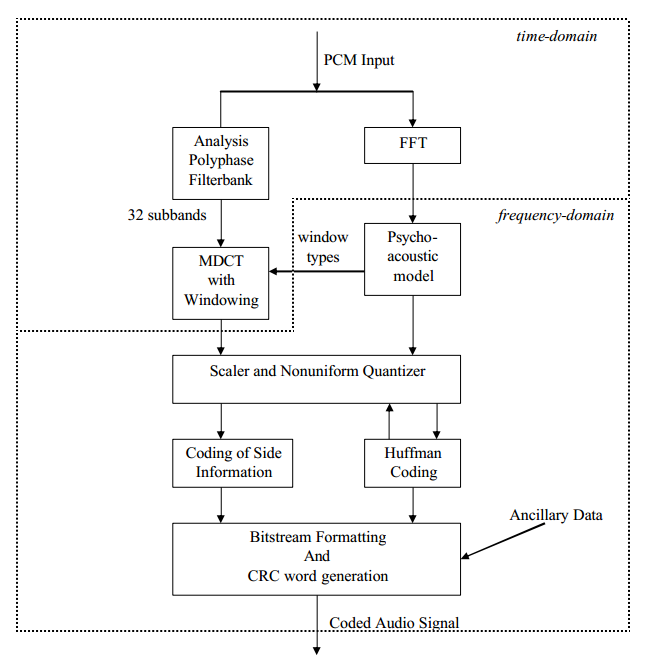
\includegraphics[scale=0.8]{encode_layout.png}
		\caption{Schema della codifica MP3.}
		\label{fig:encode_layout}
	\end{figure}
	
	Di seguito verranno illustrate le varie fasi, senza tuttavia entrare troppo nel dettaglio o in ambito implementativo.
	
	\section{Banco filtri ibrido}
		
		Il primo passo della codifica MP3 consiste nel suddividere i sample PCM in sottobande e nel mapparli in sample a dominio di frequenza. Questo procedimento, detto \textit{banco filtri ibrido}, è composto da un \textit{banco filtri di analisi polifasico} e dall'algoritmo \textit{MDCT}.
		
		\subsection{Banco filtri di analisi polifasico} \label{subsec:banco_filtri_analisi_polifasico}
			
			La prima fase consiste in un banco di filtri di analisi polifasico, che prende in input 1152 sample PCM e restituisce come output 1152 sample divisi in 32 sottobande equispaziate, ovvero suddivide il segnale di input nelle sue componenti raggruppate per sottobanda. Gli estremi delle 32 sottobande sono definiti dalla sampling frequency utilizzata per ottenere i campioni PCM e dal limite di Nyquist corrispondente: se ad esempio la frequenza di campionamento è 44.1 \textit{kHz}, le frequenze campionate vanno da 0 a 22.05 \textit{kHz}, quindi ogni sottobanda sarà larga $22050/32\approx 689$ \textit{Hz}. Le sottobande saranno in questo caso 0-689 \textit{Hz}, 689-1378 \textit{Hz}, 1378-2067 \textit{Hz}, ecc\dots.
			
			\begin{wrapfigure}{r}{0.5\textwidth}
				\centering
					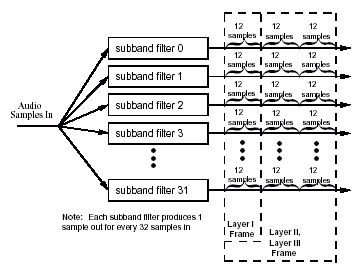
\includegraphics[scale=1]{filterbank.png}
				\caption{Banco filtri di analisi polifasico.}
				\label{fig:filterbank}
			\end{wrapfigure}
			
			Dal momento che, virtualmente, ogni sample PCM può contenere componenti di ogni sottobanda, il banco di filtri di analisi produce, di fatto, 32 sample (uno per ogni sottobanda) per ogni sample PCM, aumentando il numero di sample di un fattore 32. Quindi viene eseguito un \textit{downsampling} (o \textit{decimazione}) di fattore 32 (ovvero si prende un sample ogni 32), in modo da avere nuovamente 1152 sample. Ovviamente, il downsampling inserisce dell'aliasing (è quindi un procedimento lossy).\\
			Il banco filtri di analisi polifasico è costruito mettendo in parallelo 32 filtri passa-banda, ognuno destinato a far passare soltanto le frequenze appartenenti alla sottobanda corrispondente. Ogni sottobanda sarà composta da 36 (=1152/32) sample, suddivisi in 3 gruppi da 12, come mostrato in Figura \ref{fig:filterbank}.
		
		\subsection{MDCT} \label{subsec:MDCT}
		
			Applicando una \textit{Trasformata Discreta del Coseno Modificata} (\textit{MDCT}, \textit{Modified Discrete Cosine Transform}) ognuna delle 32 sottobande viene suddivida in 18 sottobande più fini, andando a formare un granulo di 576 linee di frequenza (anche se di fatto sono bande di frequenza, l'ampiezza di banda è talmente fine che vengono spesso chiamate linee di frequenza). Inoltre, essendo un tipo particolare di Trasformata Discreta del Coseno, e quindi della Trasformata di Fourier, i sample in input a dominio di tempo vengono trasformati in coefficienti a dominio di frequenza.\\
			L'MDCT prende in input i 1152 sample generati dal banco filtri di analisi polifasico (corrispondenti ad un frame, o due granuli) e produce in output 576 ($=32\cdot 18$) linee di frequenza (corrispondenti a un granulo). La MDCT si basa sulla sovrapposizione degli input (a due a due) per produrre gli output, secondo lo schema in Figura \ref{fig:mdct}.\\
			
			\begin{figure}[h!]
				\centering
					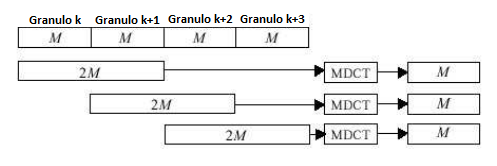
\includegraphics[scale=1]{mdct.png}
				\caption{Trasformazione MDCT.}
				\label{fig:mdct}
			\end{figure}
			
			In generale, la MDCT prende in input $2N$ sample $\{y_n\}$, $n=0,\dots,2N-1$, e restituisce in output $N$ sample a dominio di frequenza $\{x_k\}$, $k=0,\dots,N-1$, secondo la seguente formula:
			
			\begin{equation} \label{eqn:mdct}
				x_k = \sum_{n=0}^{2N-1}y_n\cdot\cos\left[\frac{\pi}{N}\left(n+\frac{1}{2}+\frac{N}{2}\right)\left(k+\frac{1}{2}\right)\right], \qquad k=0,\dots,N-1.
			\end{equation}
			
			Prima di applicare la MDCT è tuttavia necessario utilizzare una funzione di finestra per eliminare (assieme alla MDCT) gli artefatti temporali durante una transizione di frame. Lo standard MP3 definisce quattro tipi di finestre (Figura \ref{fig:windows}), a seconda della stazionarietà del modello psicoacustico.\\
			
			\begin{figure}[h!]
				\centering
					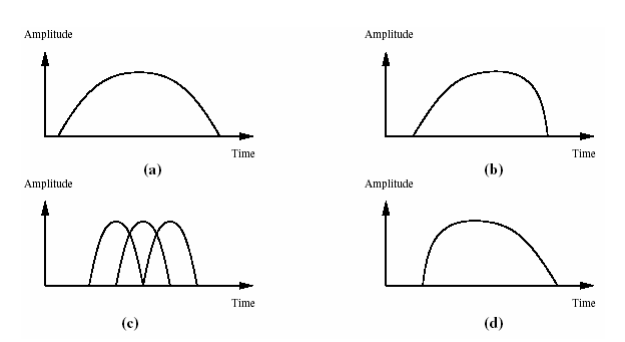
\includegraphics[scale=1]{windows.png}
				\caption[Tipologie di finestre.]{Tipologie di finestre: (a) finestra lunga; (b) finestra inizio; (c) 3 finestre corte; (d) finestra fine.}
				\label{fig:windows}
			\end{figure}
			
			Se il modello psicoacustico decide che (per ogni sottobanda) il segnale non cambia, o cambia poco, tra il frame corente e quello precedente, allora viene utilizzata una \textit{finestra lunga}, che migliora la risoluzione spettrale (ovvero sulla frequenza) data dall'MDCT. Se al contrario vi sono notevoli differenze, allora vengono utilizzate \textit{tre finestre corte} (sovrapposte) per migliorare la risoluzione temporale data dall'MDCT e quindi eliminare gli artefatti temporali.\\
			Quando si passa da una finestra lunga a finestre corte, si utilizza una \textit{finestra inizio}. Viceversa, se si passa da finestre corte ad una finestra lunga si utilizza una \textit{finestra fine}.\\
			In concreto, l'applicazione della funzione finestra consiste nel moltiplicare ogni input per una funzione seno (a seconda della finestra utilizzata).\\
			\\
			Come già accennato, la decimazione fatta dal banco di filtri di analisi polifasico introduce dell'aliasing, ma permette di inviare meno informazioni. L'aliasing in questione verrà ridotto in fase di decodifica tramite calcoli ``a farfalla'', come vedremo nel Capitolo \ref{chap:decodifica}.
			
	\section{Fast Fourier Transform} \label{sec:fft}
		
		Dal momento che la risoluzione di frequenza data dal banco filtri è troppo bassa, simultaneamente al banco filtri di analisi polifasico viene effettuata una \textit{Trasformata di Fourier veloce}, o \textit{Fast Fourier Transform} (\textit{FFT}), in modo da avere una miglior risoluzione e più informazioni sul cambiamento di frequenza nel tempo. La FFT (che non è altro che una versione ottimizzata della Trasformata Discreta di Fourier) mappa il segnale in entrata a dominio di tempo in un segnale a dominio di frequenza. In questo caso viene utilizzata una FFT a 1024 o 256 punti su 1152 sample PCM in entrata.
		
	\section{Modello psicoacustico} \label{sec:modello_psicoacustico}
		
		Questa fase rappresenta il modello psicoacustico. Esso prende in input i sample, a dominio di frequenza, generati dalla FFT e fornisce informazioni all'MDCT su quale finestra utilizzare. Inoltre da anche informazioni alla fase di Quantizzazione Non Uniforme su come quantizzare le diverse linee di frequenza.\\
		\\
		Per decidere quale finestra inviare all'MDCT, vengono comparati gli spettri del frame corrente e del frame precedente. Se non vengono rilevati cambiamenti (\textit{no attack}) allora si utilizza una finestra lunga. Se vengono registrati cambiamenti (\textit{attack}), viene effettuato il passaggio da finestra lunga a finestre corte e quest'ultime verranno utilizzate finché il segnale non si stabilizzerà nuovamente. In Figura \ref{fig:psychoacoustic_model} è rappresentato il diagramma di decisione della finestra da inviare all'MDCT.\\
		
		\begin{figure}[h!]
			\centering
				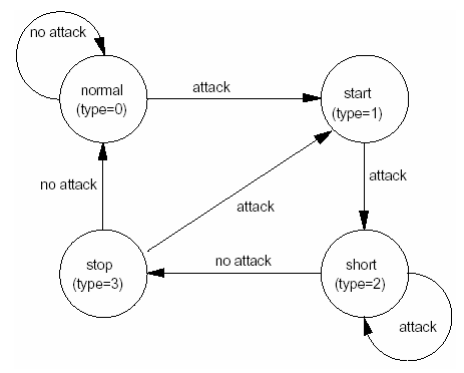
\includegraphics[scale=1]{psychoacoustic_model.png}
			\caption{Modello psicoacustico: diagramma di decisione della finestra.}
			\label{fig:psychoacoustic_model}
		\end{figure}
		
		Il modello psicoacustico, inoltre, analizza lo spettro fornito dalla FFT per indiciduare le componenti dominanti e calcolare la soglia di mascheramento per ogni banda critica (le frequenze sotto questa soglia verranno mascherate). Le soglie di mascheramento di ogni banda critica verranno quindi utilizzate nella Quantizzazione Non Uniforme per diminuire il rumore di quantizzazione.
		
	\section{Quantizzazione Non Uniforme} \label{sec:quantizzazione_non_uniforme}
		
		In questa fase vengono scalati e quantizzati 576 sample a dominio di frequenza per volta. Lo schema generale presenta due cicli annidati: \textit{rate control loop} (ciclo di controllo del tasso, esterno) e \textit{distorsion control loop} (ciclo di controllo della distorsione, interno).
		
		\begin{itemize}
			\item \textit{rate control loop}: in questo ciclo avviene la quantizzazione dei sample. I valori vengono quantizzati più volte, con step di quantizzazione sempre maggiori, fino a che i valori quantizzati non possono essere codificati con una delle tabelle di Huffman disponibili (step di quantizzazione più grandi implicano valori quantizzati più piccoli). Quindi viene calcolata la somma dei bit utilizzati per i valori quantizzati codificati con Huffman: se i bit necessari rientrano nei bit disponibili, allora si passa al loop interno, altrimenti si ripete il processo aumentando lo step di quantizzazione finché i bit disponibili non sono sufficienti. In questo step, inoltre, vengono calcolate anche le regioni e sottoregioni (big values, count1, rzero, ecc\dots) ed i rispettivi limiti. Lo step di quantizzazione viene regolato dal campo global\_gain nella Side Information di ogni granulo (vedi Capitolo \ref{chap:struttura_file_mp3}).
			
			\item \textit{distorsion control loop}: in questo ciclo, invece, viene controllato il rumore di quantizzazione prodotto nel ciclo precedente e vengono quindi aggiustati i fattori di scala finché il rumore non è mascherato per ogni banda di fattori di scala. Si applicano quindi i fattori di scala ad ogni linea di frequenza di ogni banda di fattori di scala, finché tutte le bande di fattori di scala non hanno il rumore inferiore alla soglia di mascheramento calcolata per quella banda (dal modello psicoacustico). Se una banda presenta un rumore di quantizzazione maggiore della soglia di mascheramento, allora il rumore sarà udibile dall'orecchio umano: in questi casi il fattore di scala corrispondente viene aumentato (maggiore è il fattore di scala, meno viene scalato il sample) e il processo ripetuto. Quando finalmente tutte le bande di fattori di scala saranno poco rumorose (ovvero con rumore sotto la soglia di mascheramento) si uscirà dal ciclo di controllo di distorsione, salvando fattori di scala e step di quantizzazione, per entrare nuovamente nel ciclo esterno, in modo da poter utilizzare step di quantizzazione più piccoli (se possibile) con i nuovi valori scalati.
			
		\end{itemize}
		
	\section{Codifica Huffman} \label{sec:codifica_huffman}
		
		Una volta terminata la quantizzazione e la determinazione dei fattori di scala, i valori quantizzati vengono codificati con la tabella di Huffman corrispondente (a seconda delle tabelle scelte per le varie regioni e sottoregioni). Si osservi che, prima della codifica di Huffman, vengono riordinate le linee di frequenza relative alle finestre corte prima per sottobanda, poi per frequenza ed infine per finestra, in quanto sample con frequenza simile hanno più probabilità di avere valori simili (l'output dell'MDCT ordinava questi sample per sottobanda, per finestra e quindi per frequenza).
		
	\section{Strutturazione della Side Information} \label{sec:strutturazione_side_information}
		
		A questo punto tutti i dati generati nelle fasi precedenti (step di quantizzazione, tabelle di huffman, finestre, ecc\dots) vengono strutturati secondo il formato visto per la Side Information, essendo necessari per la decodifica del file \texttt{.mp3}.
		
	\section{Formattazione del flusso di bit} \label{sec:formattazione_flusso_bit}
		
		A questo punto l'encoder MP3 è in possesso di tutti i dati necessari: l'header, la CRC, la Side Information e i dati principali vengono messi insieme e strutturati secondo il formato visto nel Capitolo \ref{chap:struttura_file_mp3}. Il risultato è un frame MP3, corrispondente a 1152 sample PCM, ovvero a 26 \textit{ms} di audio\footnote{A 44.1 \textit{kHz} di frequenza di campionamento.}.
		